\documentclass[a4paper,12pt]{article}

% > Page setup
\usepackage[left=2.25cm, right=2.25cm, top=2.5cm, bottom=2.5cm]{geometry}
\usepackage{setspace}       		% line spacing
\usepackage{graphicx}       		% image support
\graphicspath{{resources/}} 		% image folder
\doublespacing              		% double spacing
\renewcommand{\arraystretch}{0.6}	% since the forced double spacing ruins everything
\pagenumbering{arabic}      		% page numbering

% > Math packages
\usepackage{physics}							% well, it's a physics package but whatever
\usepackage{amsmath, amssymb, amsfonts, amsthm} % math symbols & environments

% > References & bibliography
\usepackage{cite}                                  % BibTeX citation support
\usepackage[notlof,nottoc,numbib]{tocbibind}       % include bibliography in ToC

% > Styling & utilities
\usepackage{xcolor} % colored text

% > Custom commands

% fix ugly Nabla physics package operators
\renewcommand\gradient[1]{\nabla#1}
\renewcommand\divergence[1]{\nabla\vdot#1}
\renewcommand\curl[1]{\nabla\cp#1}

% Vectors and symbols
\newcommand{\ihat}{\hat{\imath}}
\newcommand{\jhat}{\hat{\jmath}}
\newcommand{\rhat}{\hat{r}}
\newcommand{\nhat}{\hat{n}}
\newcommand{\thetahat}{\hat{\theta}}
\newcommand{\fatf}{\mathbf{F}}         		% vector field F
\newcommand{\fatomega}{\boldsymbol{\omega}} % vorticity
\renewcommand{\theta}{\vartheta}      		% use vartheta for theta

% Derivatives
\newcommand{\der}[2]{\frac{\mathrm{d} #1}{\mathrm{d} #2}}           % total derivative
\newcommand{\partialder}[2]{\frac{\partial #1}{\partial #2}}        % partial derivative
\newcommand{\materialder}[2]{\frac{\mathrm{D} #1}{\mathrm{D} #2}}   % material derivative

% Miscellaneous
\newcommand{\justify}[1]{\text{\color{gray}(#1)}} 								% inline justification notes
\newcommand{\definedas}{\stackrel{\Delta}{=}}     								% "defined as" symbol
\newcommand{\referto}[1]{\textsuperscript{\color{darkgray}\tiny[see \ref{#1}]}}	% citation command
\newcommand{\needcitation}{\textsuperscript{\normalfont[Citation needed]}}		% temporarily mark where I need to cite
\renewcommand{\qedsymbol}{\hfill\ensuremath{\blacksquare}}						% make the QED symbol great again
\newcommand{\vecpadding}{\vspace*{0.15cm}}										% for when fractions et cetera get too close in a vector

% Research question
\newcommand{\researchquestion}
{
	How can vector calculus be applied to model and analyze 
	incompressible fluid flow in two-dimensional spaces with 
	circular obstacles, and what mathematical insights
	does this provide about real-world fluid systems?
}

% > Theorems
\newtheorem{theorem}{Theorem}[section]
\newtheorem{corollary}{Corollary}[theorem]
\newtheorem{lemma}[theorem]{Lemma}

\begin{document}

% > Title page
\begin{titlepage}
	\begin{center}
		\vspace*{0.5cm}
		\Large\textbf{\researchquestion}

		\vspace{1.5cm}
		\large\textbf{Mathematics AA HL}

		\vfill
		\color{darkgray} Word Count: ****
	\end{center}
\end{titlepage}

% > Table of contents
\tableofcontents\newpage

% > Introduction
\section{Introduction}
Vector calculus provides the foundation and tools for the analysis and modeling of several real-world phenomona, and is integral to understanding several important fields such as aero- \& hydrodynamics, as well as the modeling of weather \& climates. 

Through the use of pure mathematics, this essay will investigate the flow of fluids in 2 dimensional spaces around circular obstacles. Visual representations through mediums such as vector field plots (plotted through a custom program
% Aim & scope
\subsection{Aim \& scope}
This essay will for simplicity's sake only cover fluid flow around circular obstacles in $\mathbb{R}^2$ spaces; an alaysis of fluid flow in $\mathbb{R}^3$ spaces would be much more complex.
Furthermore, only incompressible fluids sans sinks and sources ($\fatf\ni\divergence\fatf=0$), will be analyzed.

Most of the analysis will take place using Green's theorem\referto{sec:greenstheorem}.

% Background
\subsection{Background}
\subsubsection{Notation}
In this paper, the gradient, divergence and curl operators will be denoted using their explicit $\nabla$ forms as follows:
$$\begin{matrix}
	\mathrm{grad}\ \fatf&\equiv&\grad{\fatf}\\
	\mathrm{div}\ \fatf&\equiv&\divergence\fatf\\
	\mathrm{curl}\ \fatf&\equiv&\curl\fatf
\end{matrix}$$
The directional vector will also be denoted using $\nabla$ as $\nabla_{\vec{v}}\fatf$.

For the purposes of clarity, vectors in cartesian systems will be denoted $\begin{pmatrix}x\\y\end{pmatrix}$ whilst vectors in polar systems will be denoted as $\langle r,\theta\rangle$

To ensure point-uniqueness, all polar coordinates will be within the restrictions $r\geq0,\,\theta\in[0,2\pi)$.

\section{Mathematical background}
\subsection{The fundementals of vector calculus}
One dimensional calculus provides the tools for finding the slope of some function $f$ with respect to some variable $x$ at some point through the derivative, often denoted by Leibniz's notation $\der{f}{x}$, representing the ratio between some small change in $f$ after some small change in $x$. For example, the equation of the slope of the function $f(x)=x^2$ at some point can be calculated using the formal definition of a deriative:
\begin{equation}
	\der{f}{x}=\underbrace{\lim_{h\rightarrow0}\frac{f(x+h)-f(x)}{h}}_\text{\hidewidth The formal definition of a derivative\hidewidth}\\
\end{equation}
\begin{align*}
	f(x)=x^2\rightarrow\der{f}{x}&=\lim_{h\rightarrow0}\frac{(x+h)^2-(x)^2}{h}\\
	&=\lim_{h\rightarrow0}\frac{x^2+2xh+h^2-x^2}{h}\\
	&=\lim_{h\rightarrow0}\frac{2xh+h^2}{h}\\
	&=\lim_{h\rightarrow0}2x+h=2x
\end{align*}
More conveniently, Lagrange's or Euler's notation for the derivative is often used to avoid excessive writing.
$$\der{f}{x}\equiv f'(x)\equiv \mathrm{D}f$$
For the purposes of this essay, the formal definition of a derivative will not be used to calculate each derivation, rather common patterns and rules (such as the power rule, product rule, etc.) will be used. 

Multi-variable calculus introduces the partial derivative, which functions the same as a normal derivative but treats all variables except for the one being differentiated by as constants, allowing for the derivation of multi-variable functions.
\begin{align*}
	f(x,y)=x^2+y^2\implies\partialder{f}{x}=2x && \justify{power rule}
\end{align*}
However, the partial derivative only provides part of the picture, since it only takes into consideration one variable. Defining one single full picture "derivative" of a multi-variable function is not possible, since there are an infinite number of "slopes" at some point, and what you want the derivative to achieve will depend on your goal (e.g. what direction you want to differentiate in).

\subsubsection*{The nabla operator}
The nabla operator, denoted $\nabla$ (pronounced nabla or del), is a vector filled with partial derivatives with respect to each variable some function $f$ takes. For example, consider some function $f:\mathbb{R}^n\rightarrow\mathbb{R}^m$, nabla would then be defined as:
\begin{equation}
	\left.\nabla=
	\begin{bmatrix}
		\partialder{}{x} \\
		\partialder{}{y} \\
		\partialder{}{z} \\ 
		\vdots 	         \\
	\end{bmatrix}
	\color{gray}\right\} \color{gray}n\text{ times}\color{black}
\end{equation}
Nabla gives the vector pointing in the direction of greatest ascent\referto{p:nablagreatestchange}. For example, aplying this to our previous example $f(x,y)=x^2+y^2$ results in:
$$\nabla f=\begin{bmatrix}
	\partialder{}{x}x^2+y^2\\
	\partialder{}{y}x^2+y^2	
\end{bmatrix}=\begin{bmatrix}
	2x\\
	2y
\end{bmatrix}$$
Meaning that at some point $(x,y)$, the direction of steepest incline will be:$$2{\begin{bmatrix}x\\y\end{bmatrix}}$$
The gradient of a function is often visualized as a vector field, plotting the vector field of the previous example yields:

\begin{figure}[!ht]
	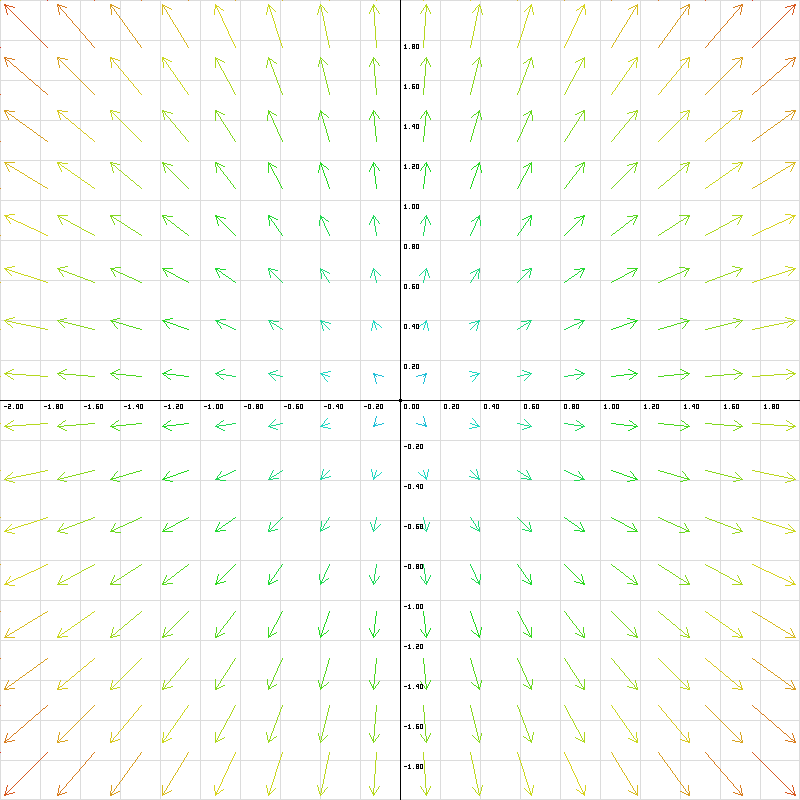
\includegraphics[scale=0.45]{x2y2.png}
	\centering
	\caption{Vector field for $f(x,y)=\begin{bmatrix}2x\\2y\end{bmatrix}$}
	\label{fig:x2y2}
\end{figure}

The nabla operator proves foundational to several important concepts within vector calculus, as will be demonstrated.

\subsubsection*{Directional derivatives}
Partial derivatives allow for the computation of derivatives in the $x$ and $y$, and this concept may be extended to the derivative in any direction $\vec{v}$. Since $\nabla f$ computes the rate of change in the $x$ and $y$ directions, dotting this vector with some directional vector $\vec{v}$ gives the directional derivative in the direction of $\vec{v}$, denoted as:
\begin{equation}
	\nabla_{\vec{v}}f=\nabla f\cdot\vec{v}
\end{equation}
Nabla pointing in the direction of greatest ascent can be proven using the directional derivative.
\begin{proof}\label{p:nablagreatestchange}
	\begin{align*}
		\nabla_{\vec{v}}f&=\nabla f\cdot\vec{v}\\
		\max\nabla_{\vec{v}}f&\rightarrow\text{direction of greatest change}\\
		\max\nabla_{\vec{v}}f&=\max\nabla f\cdot\vec{v}\\
		&=\max\lVert\nabla f\rVert\lVert\vec{v}\rVert\cos{\theta}\\
		&\leadsto\theta=0\\
		&\implies\max\nabla_{\vec{v}}f\text{ points in the direction of }\nabla f
	\end{align*}
\end{proof}
\subsubsection*{Other}
$$f:\mathbb{R}^n\rightarrow\mathbb{R}^n\ni n>1,n\in\mathbb{Z}$$
\begin{equation}
	\materialder{f}{t}\definedas\partialder{f}{t}+\underbrace{\vec{v}\cdot\nabla f}_{\hidewidth\text{Directional derivative }\nabla_{\vec{v}}f\hidewidth}
\end{equation}
$$\vec{v_1}\otimes\vec{v_2}$$

% > fluid dynamics
\subsection{Incompressible flow}
An incompressible fluid is any fluid such that $\divergence\fatf=0$, which is to say that the divergence of the fluid is 0.

\subsection{Complex analysis in 2D potential flow}

% > the navier-stokes equations
\subsection*{Green's theorem}\label{sec:greenstheorem}
\begin{equation} % navier-stokes
	\materialder{f}{\mathbf{t}}=\iiint\limits_{V}(\materialder{\rho}{\mathbf{t}}+\rho(\nabla\cdot u))dV
\end{equation}
Lorem ipsum dolor sit amet \cite{peyret2012computational}

\section{Modeling flow around circular obstacles}
\subsection{Ideal potential flow model}
\subsection{Effect of circulation on flow patterns}
\section{Real-world observations}
\section{Conclusion}

% references
\newpage
\bibliographystyle{apalike}
\bibliography{sources}
\stepcounter{section}
\addcontentsline{toc}{section}{\protect\numberline{\thesection}List of Figures}
\renewcommand{\listfigurename}{\thesection\hspace{20pt}List of Figures}\listoffigures

% testing
\newpage
\section{Research}
\subsection{Potential flow around a circular cylinder}
A cylinder of radius $L$ is placed in two-dimensional, incompressible, inviscid flow which flows in the direction of $\ihat$.
Far away from the cylinder the velocity field $\mathbf{V}$ can be described as: 
\begin{equation}\label{equation:in-infinitum}
	\mathbf{V}=U\ihat
\end{equation}
Where $U$ is some constant. Since the cylinder is impermissible, at the boundary $\mathbf{V}\cdot\nhat=0$ where the vector $\nhat$ is the unit vector normal to the surface. 

Since in this model the viscocity $\nu=0$, the flow can be modeled using the Euler equations. If the Euler equations, apply, so does Kelvin's theorem:
\begin{theorem}[Kelvin's circulation theorem]
	The circulation around a closed material loop moving with an inviscid, barotropic fluid in the presence of conservative body forces remains constant over time.\needcitation
	
	If $\Gamma$ denotes the circulation around a material loop $C(t)$ moving with the fluid, then:
	$$\materialder{\Gamma}{t}=0$$
\end{theorem}

\textit{Id est}, if the vorticity of $\mathbf{V}$ is $0$ initialy, it must remain $0$ everywhere, thus $\curl\mathbf{V}=0$. Since the flow is irrotational, $\mathbf{V}$ can be expressed as $\mathbf{V}=\nabla\phi$, where $\phi$ is the velocity potential.

Furthermore, if $\mathbf{V}$ is incompressible, that bieng that $\divergence\mathbf{V}=0$, then $\phi$ must satisfy Laplace's equation: $\Delta\phi=0$.

\subsection{Polar coordinate boundary conditions}
\subsubsection{$\mathbf{V}=U\ihat$}\label{sec:vuihat}
In polar coordinates, the base vectors $\rhat$ and $\thetahat$ are defined as:
\begin{align*}
	\rhat&\definedas\ihat\cos\theta+\jhat\sin\theta\\
	\thetahat&\definedas-\ihat\sin\theta+\jhat\cos\theta
\end{align*}
Solving for $\ihat$ and $\jhat$ gives:
\begin{align}
	\label{poihat:1}\ihat&=\frac{\rhat-\jhat\sin\theta}{\cos\theta}\\
	\label{poihat:2}\jhat&=\frac{\thetahat+\ihat\sin\theta}{\cos\theta}
\end{align}
Substituting \ref{poihat:2} into \ref{poihat:1} and isolating $\ihat$ shows that
\begin{align}
	\notag\ihat&=\frac{\rhat-\frac{\thetahat+\ihat\sin\theta}{\cos\theta}\sin\theta}{\cos\theta}\\
	\notag&=\frac{\rhat}{\cos\theta}-\frac{\thetahat\sin\theta+\ihat\sin^2\theta}{\cos^2\theta}\\
	\notag&=\frac{\rhat}{\cos\theta}-\frac{\thetahat\sin\theta}{\cos^2\theta}-\frac{\ihat\sin^2\theta}{\cos^2\theta}\\
	\notag\implies\ihat+\frac{\sin^2\theta}{\cos^2\theta}\ihat&=\frac{\rhat}{\cos\theta}-\frac{\thetahat\sin\theta}{\cos^2\theta}\\
	\notag\ihat\left(1+\frac{\sin^2\theta}{\cos^2\theta}\right)&=\frac{\rhat}{\cos\theta}-\frac{\thetahat \sin\theta}{\cos^2\theta}\\
	\notag\ihat\left(\frac{\sin^2\theta+\cos^2\theta}{\cos^2\theta}\right)&=\frac{\rhat}{\cos\theta}-\frac{\thetahat \sin\theta}{\cos^2\theta}\\
	\notag\frac{\ihat}{\cos^2\theta}&=\frac{\rhat}{\cos\theta}-\frac{\thetahat \sin\theta}{\cos^2\theta}\\
	\label{poihat:3}\ihat&=\rhat\cos\theta-\thetahat\sin\theta\qed
\end{align}
The condition stated in \ref{equation:in-infinitum} was that \textit{in infinitum}, $\mathbf{V}=U\ihat$\,. By substituting in \ref{poihat:3}, the statement becomes in terms of $\rhat$ and $\thetahat$:
$$
	\text{as}\quad r\rightarrow\infty\,,\quad\mathbf{V}=U(\rhat\cos\theta-\thetahat\sin\theta)
$$

\subsubsection{$\mathbf{V}\cdot\nhat=0$}\label{sec:vdotnhatzero}
In polar coordinates, the base vector $\rhat$ points in the direction of positive change of $r$, that being outwards from the center. If the cylinder is assumed to be the center of the coordinate system, then $\rhat$ will always point normal to the surface of the cylinder. Therefore, at the boundary of the cylinder when $r=L$,
$$\begin{matrix}
	\mathbf{V}\cdot\rhat=0
\end{matrix}$$

\subsubsection{$\Delta\phi=0$}\label{sec:deltaphizero}
In Cartesian coordinates, the Laplacian operator $\Delta$ is defined as $\nabla\cdot\nabla$, which for the scalar field $\phi$ becomes:
\begin{gather}
	\notag\Delta\phi=\frac{\partial^2\phi}{\partial x^2}+\frac{\partial^2\phi}{\partial y^2}
\end{gather}
Translating $x$ and $y$ to polar coordinates and calculating their derivatives with respect to $r$ and $\theta$ gives:
\begin{gather}
	\notag x=r\cos\theta,\quad y=r\sin\theta\\
	\label{polap:1}\partialder{x}{r}=\cos\theta,\quad\partialder{y}{r}=\sin\theta\\
	\label{polap:2}\partialder{x}{\theta}=-r\sin\theta,\quad\partialder{y}{\theta}=r\cos\theta
\end{gather}
Consequently, by the chain rule and substitution from \ref{polap:1}:
\begin{align}
	\notag\partialder{\phi}{r}&=\partialder{\phi}{x}\partialder{x}{r}+\partialder{\phi}{y}\partialder{y}{r}\\
	\label{polap:3}&=\partialder{\phi}{x}\cos\theta+\partialder{\phi}{y}\sin\theta
\end{align}
Taking the derivative of \ref{polap:3} with respect to $r$ again gives:
\begin{align}
	\notag\frac{\partial^2\phi}{\partial r^2}&=\partialder{}{r}\partialder{\phi}{x}\cos\theta+\partialder{}{r}\partialder{\phi}{y}\sin\theta\\
	\label{polap:4}&=\partialder{}{x}\partialder{\phi}{r}\cos\theta+\partialder{}{y}\partialder{\phi}{r}\sin\theta
\end{align}
Substituting \ref{polap:3} into \ref{polap:4} gives:
\begin{align}
	\notag\frac{\partial^2\phi}{\partial r^2}&=\partialder{}{x}\left(\partialder{\phi}{x}\cos\theta+\partialder{\phi}{y}\sin\theta\right)\cos\theta+\partialder{}{y}\left(\partialder{\phi}{x}\cos\theta+\partialder{\phi}{y}\sin\theta\right)\sin\theta\\
	\notag&=\frac{\partial^2\phi}{\partial x^2}\cos^2\theta+\frac{\partial^2\phi}{\partial x\partial y}\sin\theta\cos\theta+\frac{\partial^2\phi}{\partial y\partial x}\cos\theta\sin\theta+\frac{\partial^2\phi}{\partial y^2}\sin^2\theta\\
	\label{polap:5}&=\frac{\partial^2\phi}{\partial x^2}\cos^2\theta+2\frac{\partial^2\phi}{\partial x\partial y}\sin\theta\cos\theta+\frac{\partial^2\phi}{\partial y^2}\sin^2\theta
\end{align}
Applying the same process for $\partialder{\phi}{\theta}$ with substitution from \ref{polap:2} yields:
\begin{align}
	\notag\partialder{\phi}{\theta}&=\partialder{\phi}{x}\partialder{x}{\theta}+\partialder{\phi}{y}\partialder{y}{\theta}\\
	\label{polap:6}&=-\partialder{\phi}{x}r\sin\theta+\partialder{\phi}{y}r\cos\theta
\end{align}
Taking the derivative of \ref{polap:6} with respect to $\theta$ again gives:
\begin{align}
	\notag\frac{\partial^2\phi}{\partial\theta^2}&=-\partialder{}{\theta}\partialder{\phi}{x}r\sin\theta+\partialder{}{\theta}\partialder{\phi}{y}r\cos\theta
\end{align}
Since both terms contain a product of two functions dependent on $\theta$ the product rule needs to be applied. This gives:
\begin{align}
	\notag\frac{\partial^2\phi}{\partial\theta^2}&=-\frac{\partial^2\phi}{\partial\theta\partial x}r\sin\theta-\partialder{\phi}{x}r\cos\theta+\frac{\partial^2\phi}{\partial\theta\partial y}r\cos\theta-\partialder{\phi}{y}r\sin\theta\\
	\label{polap:7}&=-r\left(\partialder{\phi}{x}\cos\theta+\partialder{\phi}{y}\sin\theta\right)+r\partialder{\phi}{\theta}\left(-\partialder{}{x}\sin\theta+\partialder{}{y}\cos\theta\right)
\end{align}
Substituting \ref{polap:6} into \ref{polap:7} gives:
\begin{align}
	\label{polap:8}\frac{\partial^2\phi}{\partial\theta^2}&=-r\left(\partialder{\phi}{x}\cos\theta+\partialder{\phi}{y}\sin\theta\right)+r\underbrace{\left(-\partialder{\phi}{x}r\sin\theta+\partialder{\phi}{y}r\cos\theta\right)\left(-\partialder{}{x}\sin\theta+\partialder{}{y}\cos\theta\right)}_{\Phi}
\end{align}
Expanding $\Phi$:
\begin{align}
	\notag\Phi&=\left(-\partialder{\phi}{x}r\sin\theta+\partialder{\phi}{y}r\cos\theta\right)\left(-\partialder{}{x}\sin\theta+\partialder{}{y}\cos\theta\right)\\
	\notag&=\left(-\partialder{\phi}{x}r\sin\theta\right)\left(-\partialder{}{x}\sin\theta\right)+\left(-\partialder{\phi}{x}r\sin\theta\right)\left(\partialder{}{y}\cos\theta\right)\\
	\notag&+\left(\partialder{\phi}{y}r\cos\theta\right)\left(-\partialder{}{x}\sin\theta\right)+\left(\partialder{\phi}{y}r\cos\theta\right)\left(\partialder{}{y}\cos\theta\right)\\
	\notag&=\frac{\partial^2\phi}{\partial x^2}r\sin^2\theta-2\frac{\partial\phi}{\partial x\partial y}r\cos\theta\sin\theta+\frac{\partial^2\phi}{\partial y^2}r\cos^2\theta
\end{align}
Substituting $\Phi$ back into \ref{polap:8} gives:
\begin{align}
	\notag\frac{\partial^2\phi}{\partial\theta^2}&=-r\left(\partialder{\phi}{x}\cos\theta+\partialder{\phi}{y}\sin\theta\right)+r\left(\frac{\partial^2\phi}{\partial x^2}r\sin^2\theta-2\frac{\partial\phi}{\partial x\partial y}r\cos\theta\sin\theta+\frac{\partial^2\phi}{\partial y^2}r\cos^2\theta\right)\\
	\notag&=r^2\left(\frac{\partial^2\phi}{\partial x^2}\sin^2\theta-2\frac{\partial\phi}{\partial x\partial y}\cos\theta\sin\theta+\frac{\partial^2\phi}{\partial y^2}\cos^2\theta\right)-r\left(\partialder{\phi}{x}\cos\theta+\partialder{\phi}{y}\sin\theta\right)\\
	\label{polap:9}&=r^2\left(\frac{\partial^2\phi}{\partial x^2}\sin^2\theta-2\frac{\partial\phi}{\partial x\partial y}\cos\theta\sin\theta+\frac{\partial^2\phi}{\partial y^2}\cos^2\theta\right)-r\partialder{\phi}{r}
\end{align}
Combining \ref{polap:5} and \ref{polap:9} yields:
\begin{align}
	\notag\frac{\partial^2\phi}{\partial r^2}+\frac{\partial^2\phi}{\partial\theta^2}&=\frac{\partial^2\phi}{\partial x^2}\cos^2\theta+2\frac{\partial^2\phi}{\partial x\partial y}\sin\theta\cos\theta+\frac{\partial^2\phi}{\partial y^2}\sin^2\theta\\
	\notag&+r^2\left(\frac{\partial^2\phi}{\partial x^2}\sin^2\theta-2\frac{\partial\phi}{\partial x\partial y}\cos\theta\sin\theta+\frac{\partial^2\phi}{\partial y^2}\cos^2\theta\right)-r\partialder{\phi}{r}\\
	\notag\implies\frac{\partial^2\phi}{\partial r^2}+\frac{1}{r^2}\frac{\partial^2\phi}{\partial\theta^2}&=\frac{\partial^2\phi}{\partial x^2}\cos^2\theta+\frac{\partial^2\phi}{\partial x^2}\sin^2\theta+\frac{\partial^2\phi}{\partial y^2}\cos^2\theta+\frac{\partial^2\phi}{\partial y^2}\sin^2\theta-\frac{1}{r}\partialder{\phi}{r}\\
	\notag&=\frac{\partial^2\phi}{\partial x^2}+\frac{\partial^2\phi}{\partial y^2}-\frac{1}{r}\partialder{\phi}{r}\\
	\notag\implies\frac{\partial^2\phi}{\partial x^2}+\frac{\partial^2\phi}{\partial y^2}&=\frac{\partial^2\phi}{\partial r^2}+\frac{1}{r}\partialder{\phi}{r}+\frac{1}{r^2}\frac{\partial^2\phi}{\partial\theta^2}\\
	\label{polap:final}\therefore\Delta\phi&=\frac{\partial^2\phi}{\partial r^2}+\frac{1}{r}\partialder{\phi}{r}+\frac{1}{r^2}\frac{\partial^2\phi}{\partial\theta^2}\qed
\end{align}

\subsection{Ad confluōrem}
Summarized, the conditions translated to polar form in sections \ref{sec:vuihat}, \ref{sec:vdotnhatzero} and \ref{sec:deltaphizero} are:
$$\begin{matrix}
	&\mathbf{V}=U(\rhat\cos\theta-\thetahat\sin\theta)\quad&\text{as}\quad&r\rightarrow\infty\vecpadding\\
	&\mathbf{V}\cdot\rhat=0\quad&\text{when}\quad&r=L\vecpadding\\
	&\dfrac{\partial^2\phi}{\partial r^2}+\dfrac{1}{r}\dfrac{\partial\phi}{\partial r}+\dfrac{1}{r^2}\dfrac{\partial^2\phi}{\partial\theta^2}=0
\end{matrix}$$


$$\qty(\dv{a}{b})$$
$$\eval{x}_{a}^{b}$$
$$\vb{F}$$
\end{document}